% Don't touch this %%%%%%%%%%%%%%%%%%%%%%%%%%%%%%%%%%%%%%%%%%%
\documentclass[10pt]{article}
\usepackage{fullpage}
\usepackage[left=1in,top=1in,right=1in,bottom=1in,headheight=3ex,headsep=3ex]{geometry}
\usepackage{graphicx}
\usepackage{float}
\usepackage{caption}
\usepackage{hyperref}

\newcommand{\blankline}{\quad\pagebreak[2]}
%%%%%%%%%%%%%%%%%%%%%%%%%%%%%%%%%%%%%%%%%%%%%%%%%%%%%%%%%%%%%%

% Modify Course title, instructor name, semester here %%%%%%%%


\title{COMP576 Final Project Proposal: Distinguish AI Generated Images}
\author{Chuxuan Yin(cy48)}
\date{Nov 2022}

%%%%%%%%%%%%%%%%%%%%%%%%%%%%%%%%%%%%%%%%%%%%%%%%%%%%%%%%%%%%%%

% Don't touch this %%%%%%%%%%%%%%%%%%%%%%%%%%%%%%%%%%%%%%%%%%%
\usepackage[sc]{mathpazo}
\linespread{1.05} % Palatino needs more leading (space between lines)
\usepackage[T1]{fontenc}
\usepackage[mmddyyyy]{datetime}% http://ctan.org/pkg/datetime
\usepackage{advdate}% http://ctan.org/pkg/advdate
\newdateformat{syldate}{\twodigit{\THEMONTH}/\twodigit{\THEDAY}}
\newsavebox{\MONDAY}\savebox{\MONDAY}{Mon}% Mon
\newcommand{\week}[1]{%
%  \cleardate{mydate}% Clear date
% \newdate{mydate}{\the\day}{\the\month}{\the\year}% Store date
  \paragraph*{\kern-2ex\quad #1, \syldate{\today} - \AdvanceDate[4]\syldate{\today}:}% Set heading  \quad #1
%  \setbox1=\hbox{\shortdayofweekname{\getdateday{mydate}}{\getdatemonth{mydate}}{\getdateyear{mydate}}}%
  \ifdim\wd1=\wd\MONDAY
    \AdvanceDate[7]
  \else
    \AdvanceDate[7]
  \fi%
}
\usepackage{setspace}
\usepackage{multicol}
%\usepackage{indentfirst}
\usepackage{fancyhdr,lastpage}
\usepackage{url}
\pagestyle{fancy}
\usepackage{hyperref}
\usepackage{lastpage}
\usepackage{amsmath}
\usepackage{layout}
\usepackage{amssymb}
\usepackage{listings}
\usepackage{hyperref}

\lhead{}
\chead{}
%%%%%%%%%%%%%%%%%%%%%%%%%%%%%%%%%%%%%%%%%%%%%%%%%%%%%%%%%%%%%%

% Modify header here %%%%%%%%%%%%%%%%%%%%%%%%%%%%%%%%%%%%%%%%%
\rhead{\footnotesize COMP 576}

%%%%%%%%%%%%%%%%%%%%%%%%%%%%%%%%%%%%%%%%%%%%%%%%%%%%%%%%%%%%%%
% Don't touch this %%%%%%%%%%%%%%%%%%%%%%%%%%%%%%%%%%%%%%%%%%%
\lfoot{}
\cfoot{\small \thepage/4}
\rfoot{}

\usepackage{array, xcolor}
\usepackage{color,hyperref}
\definecolor{clemsonorange}{HTML}{EA6A20}
\hypersetup{colorlinks,breaklinks,linkcolor=clemsonorange,urlcolor=clemsonorange,anchorcolor=clemsonorange,citecolor=black}

\begin{document}
\maketitle

\section{Introduction}

\large
In the last mouths, AI painting suddenly began to attract people's attention. With the implementation of the stable diffusion framework, AI painting
finally showed its great potential on large scale commercial usages. People who know nothing about painting could also easily use this model to generate
high quality images in just one minute. While AI painting looked really awesome, it also raised some critques, one of these is that those generated images are
very homogenized, so they are unable to substitue the hand-writting pictures. Although this is a very controversial topic, we could try to think this problem in
a different way: do AI generated images really have some features in common? While it might be a hard task for human eyes to distinguish these slight differences,
AI itself could be a good classifier. We could apply these traditional image classification models on the two different kind of images, and figure out whether
the AI generated images really have "something in common".

\vspace{10pt}

\begin{figure}[h]
\centering
  \begin{minipage}{.5\textwidth}
    \hspace{0.58\textwidth}
    
\includegraphics[width=0.4\linewidth]{miku2.png}
    \label{fig:test1}
  \end{minipage}%
  \begin{minipage}{.5\textwidth}
    \hspace{0.02\textwidth}
    
\includegraphics[width=0.4\linewidth]{miku3.jpg}
    \label{fig:test2}
\end{minipage}
\caption{Can we really distinguish which image is generated by AI?}
\end{figure}

\section{Proposed Solution and Contribution}

Although this is a rather new problem, we could still apply some mature methods in image classification. Nowadays, there are already
many great pre-trained image classification models for us to choose, such as \href{https://arxiv.org/abs/1409.1556}{VCG-16[1]}, \href{https://arxiv.org/abs/1512.03385}{ResNet50[2]} and \href{https://papers.nips.cc/paper/2012/hash/c399862d3b9d6b76c8436e924a68c45b-Abstract.html}{AlexNet[3]}. We could train these models
on our dataset. But these traditional models may perform bad on this problem since all these images may have same local features. We should instead
use some fine-grained image classification models such as \href{https://arxiv.org/abs/1406.6247}{visual attention model[4]}, or modify those regular models to make them fit this problem.
We may also need to understand the \href{https://arxiv.org/abs/2112.10752}{stable diffusion model[5]}, try to find a way to extract the common features for the images it generated.

\vspace{10pt}

\begin{figure}[h]
\centering
  \begin{minipage}{.5\textwidth}
    \hspace{0.08\textwidth}
    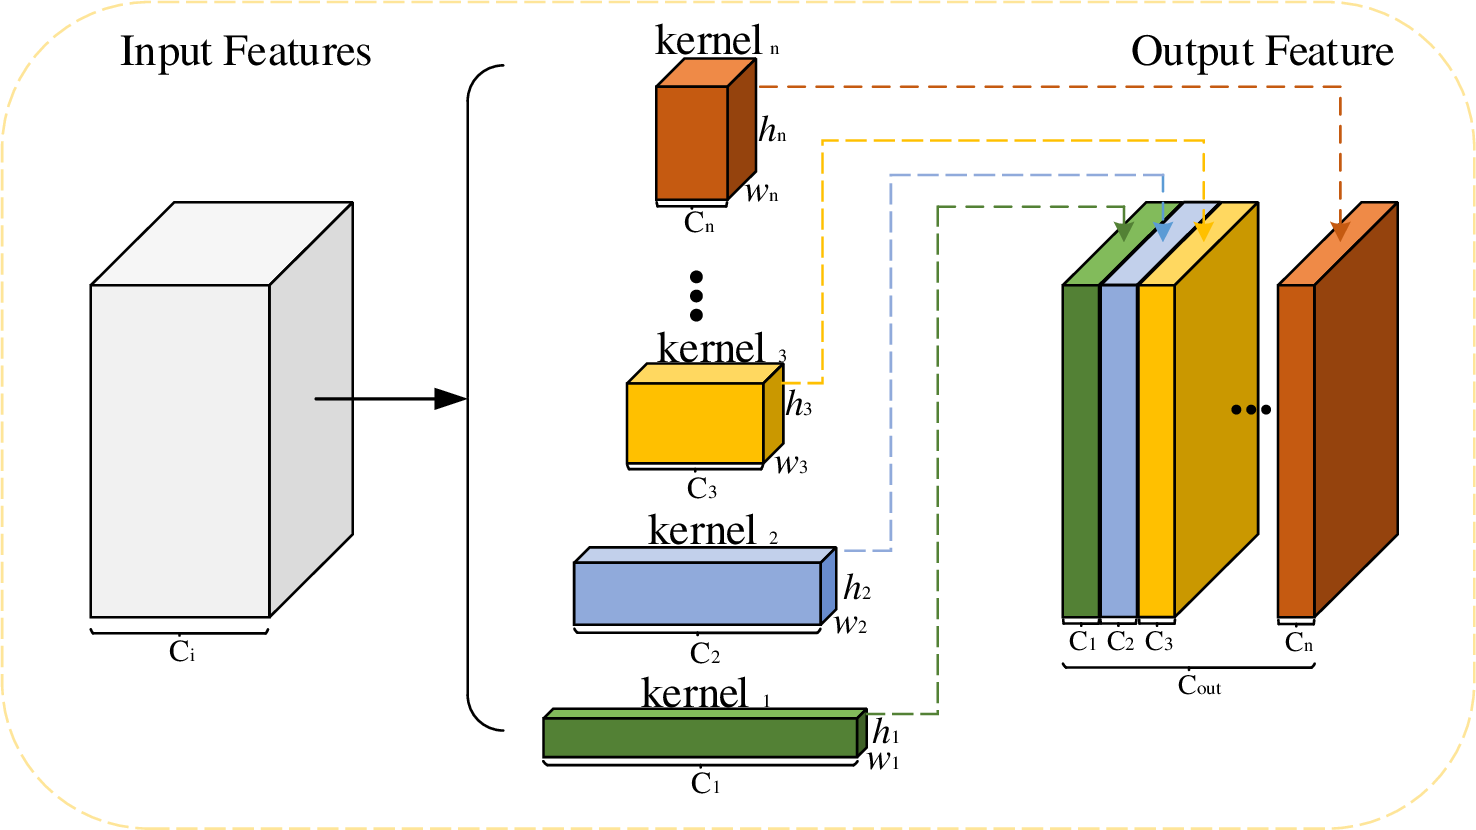
\includegraphics[width=0.9\linewidth]{fine_grained_model.PNG}
    \label{fig:test1}
  \end{minipage}%
  \begin{minipage}{.5\textwidth}
    \hspace{0.02\textwidth}
    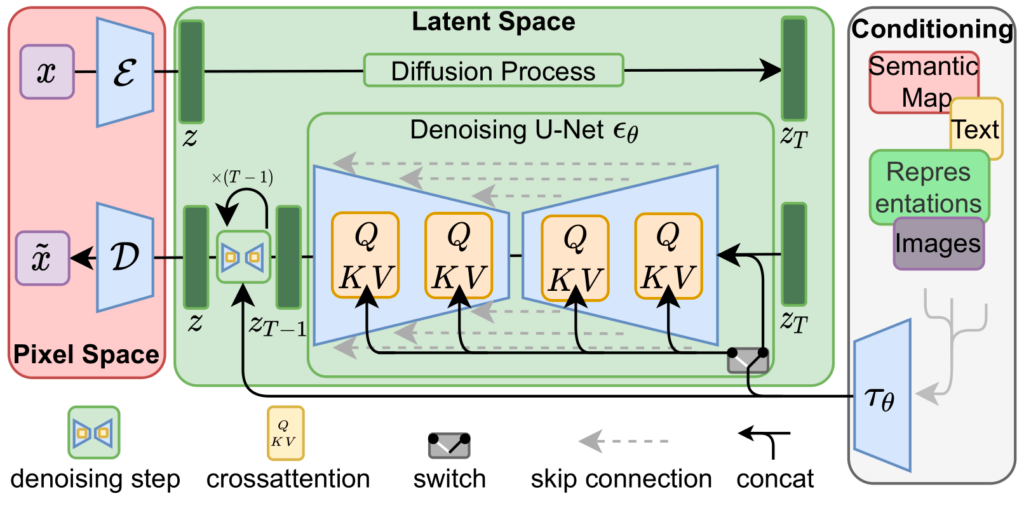
\includegraphics[width=0.9\linewidth]{stable_diffusion.png}
    \label{fig:test2}
\end{minipage}
\caption{fine grained model and stable diffusion model}
\end{figure}

\section{Goal}
The goal of this project is to find whether we could distinguish AI generated images by current image classification technique. In order to do this, we need to
try our best to build a classification model and figure out its ability. If the accuracy of prediction is greater then 60\%, then we can declare that our network could
distinguish AI generated images to some extent. Otherwise we should say even nerual network could not identify these AI generated images and we should admit they are really
good images like hand-drawings.

\vspace{10pt}

\begin{figure}[h]
\centering
  \begin{minipage}{.5\textwidth}
    \hspace{0.58\textwidth}
    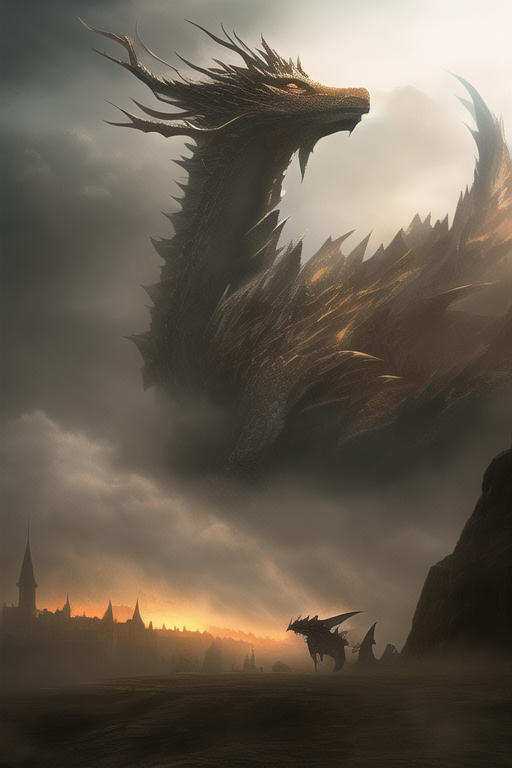
\includegraphics[width=0.4\linewidth]{good.jpg}
    \label{fig:test1}
  \end{minipage}%
  \begin{minipage}{.5\textwidth}
    \hspace{0.02\textwidth}
    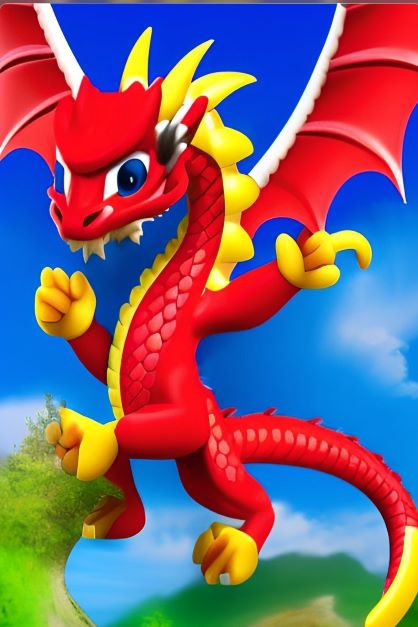
\includegraphics[width=0.4\linewidth]{bad.jpg}
    \label{fig:test2}
\end{minipage}
\caption{Good or Bad?}
\end{figure}

\section{Method}
First we need to prepare our dataset. The key issue is that we should try to make the two genre look like pretty close at a whole, so that our classification model
could mainly foucus on the tiny differences between AI generated and hand-drawings. So we will collect data based on tags: we collect images on three different kind of tags
and for each kind of tag we will give a sufficient description to restrict them in a specific scenario. We will prepere training set and testing set for each tags and test the
models' performance seperately. We will also mix them together to make a dataset, testing generalizability of the model. Considering our limited computation resources, we will preliminarily
collect 300 images on each tag, 200 for training and 100 for testing.

\vspace{10pt}

\begin{center}
  \begin{minipage}{0.3\textwidth}
    \centering
      \begin{minipage}{.5\textwidth}
        \centering
        
\includegraphics[width=0.9\linewidth]{ganyu1.jpg}
        \label{fig:test1}
      \end{minipage}%
      \begin{minipage}{.5\textwidth}
        \centering
        
\includegraphics[width=0.9\linewidth]{ganyu2.jpg}
        \label{fig:test2}
    \end{minipage}
    \captionof{figure}{Ganyu, head only}
  \end{minipage}
  \begin{minipage}{0.3\textwidth}
    \centering
      \begin{minipage}{.5\textwidth}
        \centering
        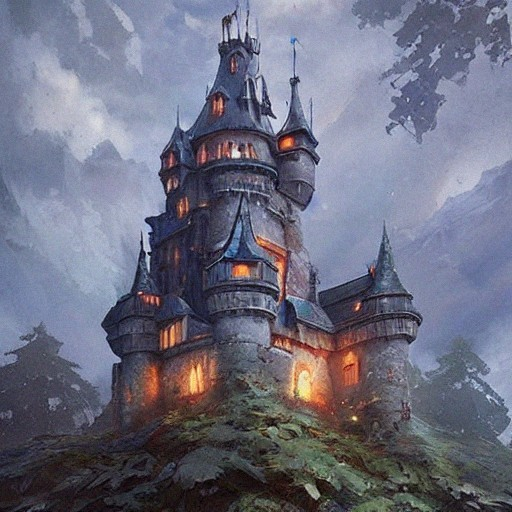
\includegraphics[width=0.9\linewidth]{castle1.jpg}
        \label{fig:test1}
      \end{minipage}%
      \begin{minipage}{.5\textwidth}
        \centering
        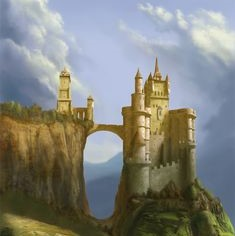
\includegraphics[width=0.9\linewidth]{castle2.jpg}
        \label{fig:test2}
    \end{minipage}
    \captionof{figure}{Castle, fantasy}
  \end{minipage}
  \begin{minipage}{0.3\textwidth}
    \centering
      \begin{minipage}{.5\textwidth}
        \centering
        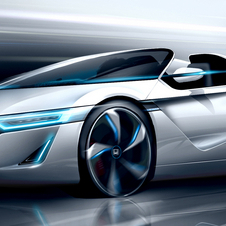
\includegraphics[width=0.9\linewidth]{sports_car1.jpg}
        \label{fig:test1}
      \end{minipage}%
      \begin{minipage}{.5\textwidth}
        \centering
        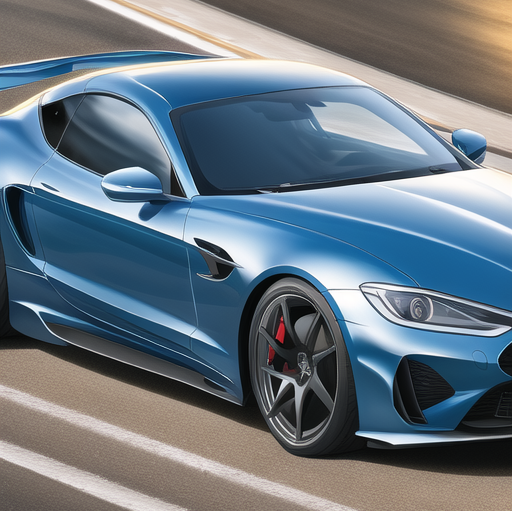
\includegraphics[width=0.9\linewidth]{sports_car2.jpg}
        \label{fig:test2}
    \end{minipage}
    \captionof{figure}{Sports car, realistic}
  \end{minipage}
\end{center}

\vspace{10pt}

Then we resize them to 200 $\times$ 200 images and put them into our classification models. We will try three different kind of models:
\begin{itemize}
  \item Fine-tuning of pre-trained image classification model, such as VCG-16
  \item Fine-grained image classification models, such as vision attetion
  \item Self-developed classification model, based on CNN
\end{itemize}

As descriped above, we will train each model on each dataset with a specific tag, and then train all the models on a generalized dataset.
Since we only care about the accuracy of prediction, the performance contrast of each model is not our interest.

\section{Feasibility}

The most challenging part of our plan is collecting data and training our model on limited computation resources. Due to these two reasons,
we choose to use 200 images in our training set and 100 images in our testing set for each tag. Laion dataset, Pixiv and Google search provide
tons of great images that we can use, while NovelAI and Wombo are good enough for generating useful AI images. With a dataset of this size,
the computation resources provided by our own laptop, RiceNots and Google Colab is enough for us to use. If we found our time and computation resources
is sufficient, we may consider to enlarge our dataset in further.

\section{Project Execution Plan}

This project will be done on one person. There are several steps we need to follow:
\begin{itemize}
  \item Design a feasible plan and write a proposal for this project
  \item Collect data from website, resize them to 200 $\times$ 200 images
  \item Survey on image classification models and stable diffusion models
  \item Implement classification models we need with tensorflow or pytorch
  \item Conduct experiment on each model for our dataset, conclude results
  \item Formulate the final report, prepare for the presentation
\end{itemize}

\section{Potential Impact}

In this project we review the AI generated images at the view of AI. It really help us understand more about AI painting, let us carefully review the difference and connection between AI painting and human painting,
which may affect how we use AI painting in the future. This project also focuses on the cutting-edge generative models and classification models. It is kind of like "generative algorithm" vs "classification algorithm",
and the result may help us figure out the limitation of each model, enhancing our understanding of them.

\begin{thebibliography}{1}
  \bibitem{Karen}
  Karen Simonyan, Andrew Zisserman. Very Deep Convolutional Networks for Large-Scale Image Recognition. \emph{arXiv:1409.1556 [cs.CV]}, Sept 2014.
  
  \bibitem{Kaiming}
  Kaiming He, Xiangyu Zhang, Shaoqing Ren, Jian Sun. Deep Residual Learning for Image Recognition. \emph{IEEE Conference on Computer Vision and Pattern Recognition}, June 2016.

  \bibitem{Alex}
  Alex Krizhevsky, Ilya Sutskever, Geoffrey E. Hinton. ImageNet Classification with Deep Convolutional Neural Networks. \emph{Advances in Neural Information Processing Systems}, May 2017.

  \bibitem{Volodymyr}
  Volodymyr Mnih, Nicolas Heess, Alex Graves and KorayKavukcuoglu. Recurrent Models of Visual Attention. \emph{Advances in Neural Information Processing Systems}, June 2014.

  \bibitem{}
  Robin Rombach, Andreas Blattmann, Dominik Lorenz, Patrick Esser and Björn Ommer. High-Resolution Image Synthesis with Latent Diffusion Models. \emph{IEEE Conference on Computer Vision and Pattern Recognition}, Dec 2021.
\end{thebibliography}
\end{document}
